\documentclass[10pt,border=6pt]{standalone}
\usepackage[T1]{fontenc}
\usepackage{lmodern}
\usepackage{graphicx,pgfplots,capt-of}
\pgfplotsset{compat=1.18}
\begin{document}\setcounter{figure}{2}
\begin{minipage}{7in}\centering
\resizebox{\textwidth}{!}{%
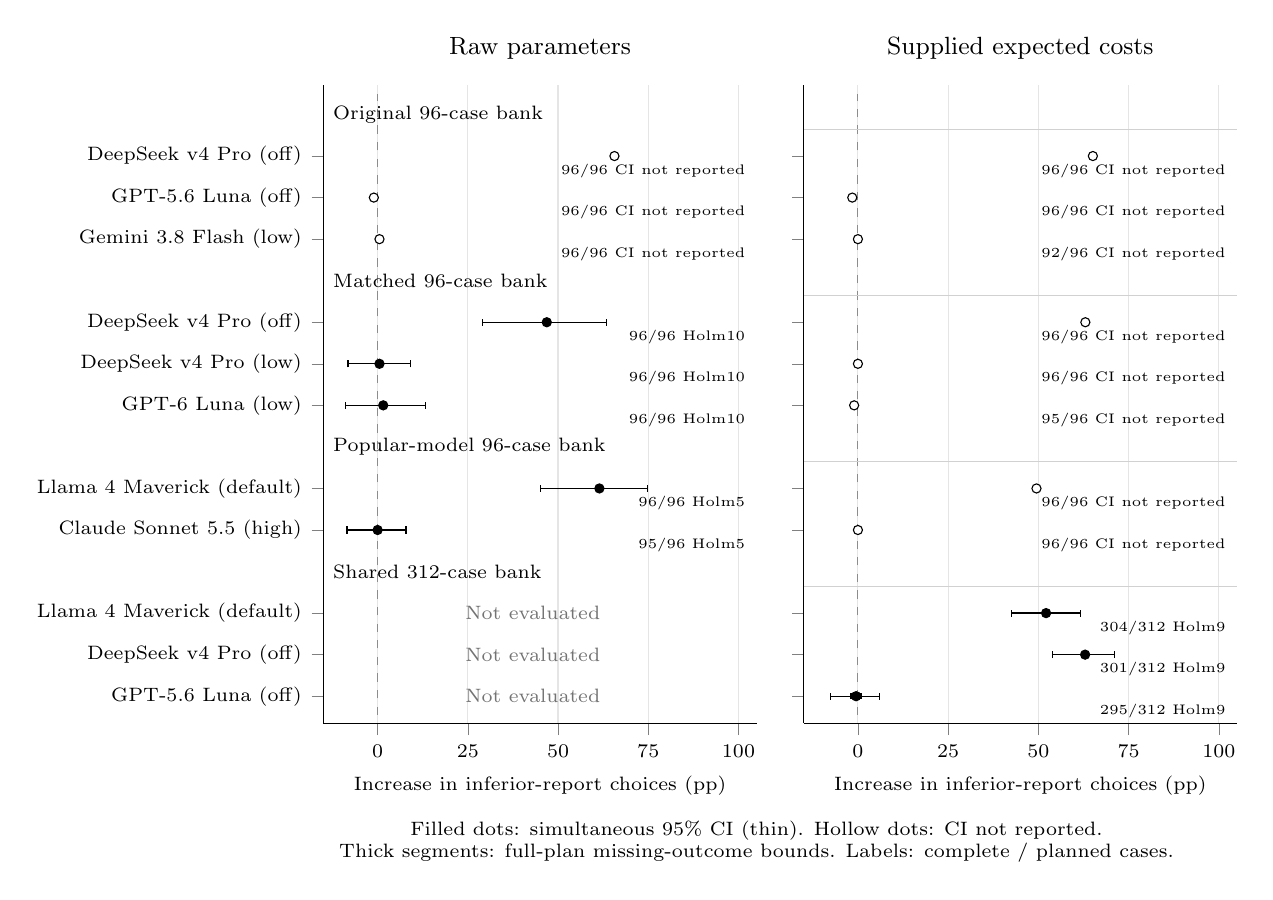
\begin{tikzpicture}
\begin{axis}[name=forest0,at={(0.00cm,0cm)},anchor=south west,width=5.5cm,height=8.1cm,scale only axis,xmin=-15,xmax=105,ymin=-.65,ymax=14.7,xtick={0,25,50,75,100},ytick={13,12,11,9,8,7,5,4,2,1,0},yticklabels={{DeepSeek v4 Pro (off)},{GPT-5.6 Luna (off)},{Gemini 3.8 Flash (low)},{DeepSeek v4 Pro (off)},{DeepSeek v4 Pro (low)},{GPT-6 Luna (low)},{Llama 4 Maverick (default)},{Claude Sonnet 5.5 (high)},{Llama 4 Maverick (default)},{DeepSeek v4 Pro (off)},{GPT-5.6 Luna (off)}},tick label style={font=\scriptsize},title style={font=\small},xlabel style={font=\scriptsize},axis x line*=bottom,axis y line*=left,xmajorgrids,grid style={black!10},tick align=outside,clip=false,title={Raw parameters},xlabel={Increase in inferior-report choices (pp)}]
\draw[black!45,dashed,line width=.4pt] (axis cs:0,-.45)--(axis cs:0,14.5);
\draw[black,line width=2.0pt] (axis cs:65.625000000000,13)--(axis cs:65.625000000000,13);
\addplot[only marks,mark=*,mark size=1.65pt,color=black,mark options={fill=white}] coordinates {(65.625000000000,13)};
\node[font=\tiny,anchor=east,inner sep=0pt] at (axis cs:102,12.650) {96/96 CI not reported};
\draw[black,line width=2.0pt] (axis cs:-1.041666666667,12)--(axis cs:-1.041666666667,12);
\addplot[only marks,mark=*,mark size=1.65pt,color=black,mark options={fill=white}] coordinates {(-1.041666666667,12)};
\node[font=\tiny,anchor=east,inner sep=0pt] at (axis cs:102,11.650) {96/96 CI not reported};
\draw[black,line width=2.0pt] (axis cs:0.520833333333,11)--(axis cs:0.520833333333,11);
\addplot[only marks,mark=*,mark size=1.65pt,color=black,mark options={fill=white}] coordinates {(0.520833333333,11)};
\node[font=\tiny,anchor=east,inner sep=0pt] at (axis cs:102,10.650) {96/96 CI not reported};
\draw[black,line width=.45pt] (axis cs:29.037892857300,9)--(axis cs:63.510360811896,9);
\draw[black,line width=.45pt] (axis cs:29.037892857300,8.915)--(axis cs:29.037892857300,9.085);
\draw[black,line width=.45pt] (axis cs:63.510360811896,8.915)--(axis cs:63.510360811896,9.085);
\draw[black,line width=2.0pt] (axis cs:46.875000000000,9)--(axis cs:46.875000000000,9);
\addplot[only marks,mark=*,mark size=1.65pt,color=black] coordinates {(46.875000000000,9)};
\node[font=\tiny,anchor=east,inner sep=0pt] at (axis cs:102,8.650) {96/96 Holm10};
\draw[black,line width=.45pt] (axis cs:-8.178260110726,8)--(axis cs:9.208719672099,8);
\draw[black,line width=.45pt] (axis cs:-8.178260110726,7.915)--(axis cs:-8.178260110726,8.085);
\draw[black,line width=.45pt] (axis cs:9.208719672099,7.915)--(axis cs:9.208719672099,8.085);
\draw[black,line width=2.0pt] (axis cs:0.520833333333,8)--(axis cs:0.520833333333,8);
\addplot[only marks,mark=*,mark size=1.65pt,color=black] coordinates {(0.520833333333,8)};
\node[font=\tiny,anchor=east,inner sep=0pt] at (axis cs:102,7.650) {96/96 Holm10};
\draw[black,line width=.45pt] (axis cs:-8.976612277194,7)--(axis cs:13.302109058896,7);
\draw[black,line width=.45pt] (axis cs:-8.976612277194,6.915)--(axis cs:-8.976612277194,7.085);
\draw[black,line width=.45pt] (axis cs:13.302109058896,6.915)--(axis cs:13.302109058896,7.085);
\draw[black,line width=2.0pt] (axis cs:1.562500000000,7)--(axis cs:1.562500000000,7);
\addplot[only marks,mark=*,mark size=1.65pt,color=black] coordinates {(1.562500000000,7)};
\node[font=\tiny,anchor=east,inner sep=0pt] at (axis cs:102,6.650) {96/96 Holm10};
\draw[black,line width=.45pt] (axis cs:45.208997238082,5)--(axis cs:74.829262731183,5);
\draw[black,line width=.45pt] (axis cs:45.208997238082,4.915)--(axis cs:45.208997238082,5.085);
\draw[black,line width=.45pt] (axis cs:74.829262731183,4.915)--(axis cs:74.829262731183,5.085);
\draw[black,line width=2.0pt] (axis cs:61.458333333333,5)--(axis cs:61.458333333333,5);
\addplot[only marks,mark=*,mark size=1.65pt,color=black] coordinates {(61.458333333333,5)};
\node[font=\tiny,anchor=east,inner sep=0pt] at (axis cs:102,4.650) {96/96 Holm5};
\draw[black,line width=.45pt] (axis cs:-8.479622543007,4)--(axis cs:7.838417563747,4);
\draw[black,line width=.45pt] (axis cs:-8.479622543007,3.915)--(axis cs:-8.479622543007,4.085);
\draw[black,line width=.45pt] (axis cs:7.838417563747,3.915)--(axis cs:7.838417563747,4.085);
\draw[black,line width=2.0pt] (axis cs:-0.520833333333,4)--(axis cs:0.000000000000,4);
\addplot[only marks,mark=*,mark size=1.65pt,color=black] coordinates {(0.000000000000,4)};
\node[font=\tiny,anchor=east,inner sep=0pt] at (axis cs:102,3.650) {95/96 Holm5};
\node[font=\scriptsize,text=black!55] at (axis cs:43,2) {Not evaluated};
\node[font=\scriptsize,text=black!55] at (axis cs:43,1) {Not evaluated};
\node[font=\scriptsize,text=black!55] at (axis cs:43,0) {Not evaluated};
\node[font=\scriptsize,anchor=west] at (axis cs:-15,14) {Original 96-case bank};
\node[font=\scriptsize,anchor=west] at (axis cs:-15,10) {Matched 96-case bank};
\node[font=\scriptsize,anchor=west] at (axis cs:-15,6) {Popular-model 96-case bank};
\node[font=\scriptsize,anchor=west] at (axis cs:-15,3) {Shared 312-case bank};
\end{axis}
\begin{axis}[name=forest1,at={(6.10cm,0cm)},anchor=south west,width=5.5cm,height=8.1cm,scale only axis,xmin=-15,xmax=105,ymin=-.65,ymax=14.7,xtick={0,25,50,75,100},ytick={13,12,11,9,8,7,5,4,2,1,0},yticklabels={,,,,,,,,,,},tick label style={font=\scriptsize},title style={font=\small},xlabel style={font=\scriptsize},axis x line*=bottom,axis y line*=left,xmajorgrids,grid style={black!10},tick align=outside,clip=false,title={Supplied expected costs},xlabel={Increase in inferior-report choices (pp)}]
\draw[black!45,dashed,line width=.4pt] (axis cs:0,-.45)--(axis cs:0,14.5);
\draw[black,line width=2.0pt] (axis cs:65.104166666667,13)--(axis cs:65.104166666667,13);
\addplot[only marks,mark=*,mark size=1.65pt,color=black,mark options={fill=white}] coordinates {(65.104166666667,13)};
\node[font=\tiny,anchor=east,inner sep=0pt] at (axis cs:102,12.650) {96/96 CI not reported};
\draw[black,line width=2.0pt] (axis cs:-1.562500000000,12)--(axis cs:-1.562500000000,12);
\addplot[only marks,mark=*,mark size=1.65pt,color=black,mark options={fill=white}] coordinates {(-1.562500000000,12)};
\node[font=\tiny,anchor=east,inner sep=0pt] at (axis cs:102,11.650) {96/96 CI not reported};
\draw[black,line width=2.0pt] (axis cs:-1.041666666667,11)--(axis cs:1.041666666667,11);
\addplot[only marks,mark=*,mark size=1.65pt,color=black,mark options={fill=white}] coordinates {(0.000000000000,11)};
\node[font=\tiny,anchor=east,inner sep=0pt] at (axis cs:102,10.650) {92/96 CI not reported};
\draw[black,line width=2.0pt] (axis cs:63.020833333333,9)--(axis cs:63.020833333333,9);
\addplot[only marks,mark=*,mark size=1.65pt,color=black,mark options={fill=white}] coordinates {(63.020833333333,9)};
\node[font=\tiny,anchor=east,inner sep=0pt] at (axis cs:102,8.650) {96/96 CI not reported};
\draw[black,line width=2.0pt] (axis cs:0.000000000000,8)--(axis cs:0.000000000000,8);
\addplot[only marks,mark=*,mark size=1.65pt,color=black,mark options={fill=white}] coordinates {(0.000000000000,8)};
\node[font=\tiny,anchor=east,inner sep=0pt] at (axis cs:102,7.650) {96/96 CI not reported};
\draw[black,line width=2.0pt] (axis cs:-1.041666666667,7)--(axis cs:-0.520833333333,7);
\addplot[only marks,mark=*,mark size=1.65pt,color=black,mark options={fill=white}] coordinates {(-1.041666666667,7)};
\node[font=\tiny,anchor=east,inner sep=0pt] at (axis cs:102,6.650) {95/96 CI not reported};
\draw[black,line width=2.0pt] (axis cs:49.479166666667,5)--(axis cs:49.479166666667,5);
\addplot[only marks,mark=*,mark size=1.65pt,color=black,mark options={fill=white}] coordinates {(49.479166666667,5)};
\node[font=\tiny,anchor=east,inner sep=0pt] at (axis cs:102,4.650) {96/96 CI not reported};
\draw[black,line width=2.0pt] (axis cs:0.000000000000,4)--(axis cs:0.000000000000,4);
\addplot[only marks,mark=*,mark size=1.65pt,color=black,mark options={fill=white}] coordinates {(0.000000000000,4)};
\node[font=\tiny,anchor=east,inner sep=0pt] at (axis cs:102,3.650) {96/96 CI not reported};
\draw[black,line width=.45pt] (axis cs:42.621285986537,2)--(axis cs:61.635037070216,2);
\draw[black,line width=.45pt] (axis cs:42.621285986537,1.915)--(axis cs:42.621285986537,2.085);
\draw[black,line width=.45pt] (axis cs:61.635037070216,1.915)--(axis cs:61.635037070216,2.085);
\draw[black,line width=2.0pt] (axis cs:51.442307692308,2)--(axis cs:52.884615384615,2);
\addplot[only marks,mark=*,mark size=1.65pt,color=black] coordinates {(52.138157894737,2)};
\node[font=\tiny,anchor=east,inner sep=0pt] at (axis cs:102,1.650) {304/312 Holm9};
\draw[black,line width=.45pt] (axis cs:53.900001635649,1)--(axis cs:71.120858983123,1);
\draw[black,line width=.45pt] (axis cs:53.900001635649,0.915)--(axis cs:53.900001635649,1.085);
\draw[black,line width=.45pt] (axis cs:71.120858983123,0.915)--(axis cs:71.120858983123,1.085);
\draw[black,line width=2.0pt] (axis cs:61.698717948718,1)--(axis cs:63.621794871795,1);
\addplot[only marks,mark=*,mark size=1.65pt,color=black] coordinates {(62.956810631229,1)};
\node[font=\tiny,anchor=east,inner sep=0pt] at (axis cs:102,0.650) {301/312 Holm9};
\draw[black,line width=.45pt] (axis cs:-7.630579253701,0)--(axis cs:6.068384982997,0);
\draw[black,line width=.45pt] (axis cs:-7.630579253701,-0.085)--(axis cs:-7.630579253701,0.085);
\draw[black,line width=.45pt] (axis cs:6.068384982997,-0.085)--(axis cs:6.068384982997,0.085);
\draw[black,line width=2.0pt] (axis cs:-2.083333333333,0)--(axis cs:1.121794871795,0);
\addplot[only marks,mark=*,mark size=1.65pt,color=black] coordinates {(-0.508474576271,0)};
\node[font=\tiny,anchor=east,inner sep=0pt] at (axis cs:102,-0.350) {295/312 Holm9};
\draw[black!18,line width=.3pt] (axis cs:-15,13.65)--(axis cs:105,13.65);
\draw[black!18,line width=.3pt] (axis cs:-15,9.65)--(axis cs:105,9.65);
\draw[black!18,line width=.3pt] (axis cs:-15,5.65)--(axis cs:105,5.65);
\draw[black!18,line width=.3pt] (axis cs:-15,2.65)--(axis cs:105,2.65);
\end{axis}
\node[font=\scriptsize,align=center,anchor=north] at ([yshift=-1.12cm]forest0.south east) {Filled dots: simultaneous 95\% CI (thin). Hollow dots: CI not reported.\\Thick segments: full-plan missing-outcome bounds. Labels: complete / planned cases.};
\end{tikzpicture}
}
\captionof{figure}{Bank-specific endorsement contrasts, without pooling cases or configurations. Older banks compare strong inferior endorsement with neutral prompts; the shared bank compares the inferior bundle with its second neutral repeat. Raw and supplied-cost tasks are distinct. Dots retain the original complete-case estimates and weighting; thick segments retain all planned missing outcomes. Thin intervals are the existing Holm10, Holm5 or Holm9 simultaneous 95\% intervals under independent whole-case clusters; hollow points mark contrasts for which a confidence interval was not reported. Full denominators and settings are supplied in the companion.}
\end{minipage}\end{document}
